
\documentclass[12pt]{article}
\usepackage{graphicx} % for including images
\usepackage{hyperref} % for creating hyperlinks
\usepackage{amsmath} % for mathematical expressions
\usepackage{lipsum} % for generating dummy text
\usepackage{listings} % for code blocks
\usepackage{float} % place images where they appear in the LaTeX
\usepackage{pdfpages} % insert PDFs in the document

\lstset{
  language=bash,
  basicstyle=\ttfamily,
  breaklines=true
}

\begin{document}
% Title page information
\title{Sound Classification and Localization by Acoustic Sensing on Raspberry Pi 4}
\author{Jaidon Lybbert, University of Washington}
\date{January 24, 2024}

% Generate the title page
\maketitle

% Abstract section
\begin{abstract}
	In this article a network of distributed acoustic sensing nodes is used to localize a sound signature using a time-difference-of-arrival (TDoA) algorithm. Accurate wall-clock times are obtained by GPS at each node, and a frame of acoustic data is recorded through a microphone on each node. Time differences are determined by correlation, and the resulting system of equations solved by the Chan-Ho algorithm to determine location. In a concurrent process, each node performs classification inference on a data frame using a pre-trained convolutional neural network (CNN). The resulting class identification is used to assign a process model to the tracked object for use in an Extended Kalman Filter (EKF) applied to the Chan-Ho localization result to make the final estimate of object position and trajectory.
\end{abstract}

% Introduction section
\section{Introduction}
This document is organized as follows. In Section \ref{sec:background} \ref{sec:methods} \ref{sec:results} \ref{sec:discussion}. I conclude in \ref{sec:conclusion} by discussing the overall takeaways from my experiments and things I would like to try in the future.

% Methods section
\section{Background}\label{sec:background}

\section{TensorFlow Lite}

\section{Kalman Filters}

	The Extended Kalman Filter (EKF) is a well-described algorithm, where discrete samples from one or more sensors is combined with an analytic model of a system to estimate system state. A block diagram of the Kalman Filter from \textit{Kalman Filters for Beginners} by Phil Kim \cite{kim2011kalman} is shown in Fig \ref{fig:kimkalman}.
	
\begin{figure}[h]
\centering
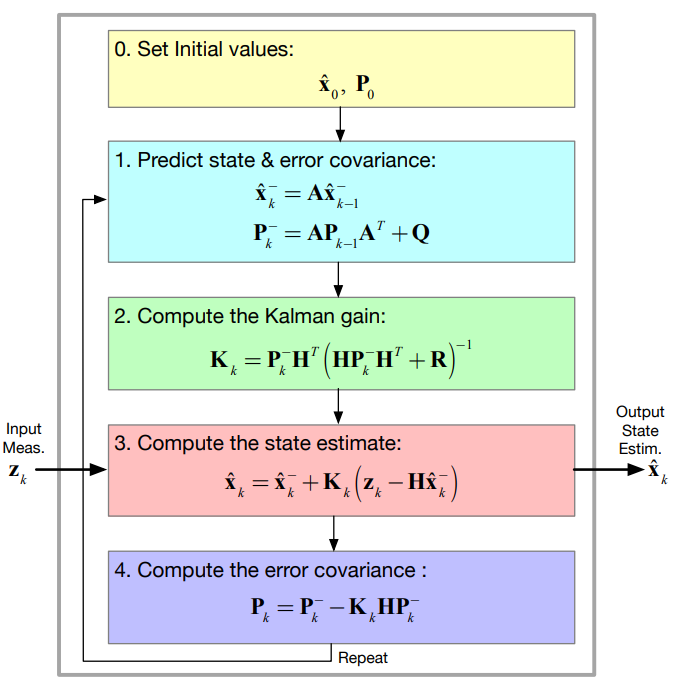
\includegraphics[width=0.5\textwidth]{kimkalman.png} % replace with your own image file
\caption{Block diagram of the Kalman Filter algorithm. $\hat{\mathbf{x}}_0$ represents the initial state.}
\label{fig:kimkalman}
\end{figure}

\section{Methods}\label{sec:methods}

\subsection{Environment Setup}

	For classification, I will be using TensorFlow Lite
	
\subsubsection{GPS}
	I used the Adafruit Ultimate GPS USB breakout board to get GPS data through \textbf{gpsd} \cite{townsend2023}.
	
\begin{lstlisting}
sudo apt install gspd gpsd-clients
sudo systemctl stop gpsd.socket
sudo systemctl disable gpsd.socket
sudo killall gpsd
sudo gpsd /dev/ttyUSB -F /var/run/gpsd.sock
\end{lstlisting}

To test the device I used the command \textbf{cgps -s}, which prints out GPS status information to the console, as shown in Fig. \ref{fig:cgps}.

\begin{figure}[h]
\centering
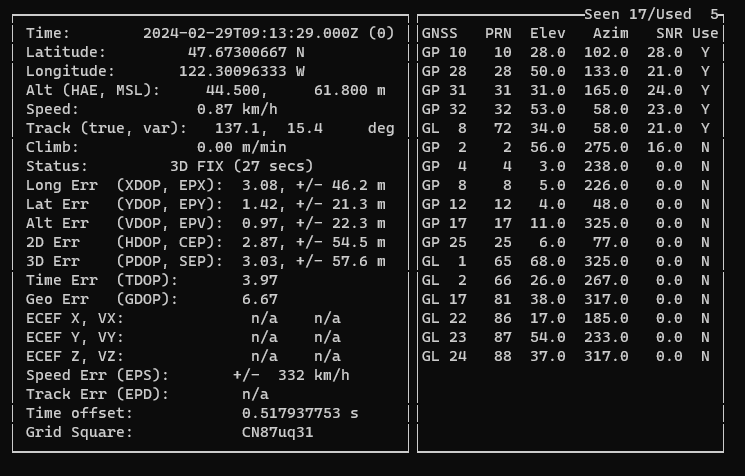
\includegraphics[width=0.8\textwidth]{cgps.png} % replace with your own image file
\caption{Terminal display of GPS information from the \textbf{cgps -s} command.}
\label{fig:cgps}
\end{figure}

% Results section
\section{Results}\label{sec:results}

% Discussion section
\section{Discussion}\label{sec:discussion}

% Conclusion section
\section{Conclusion}\label{sec:conclusion}

\paragraph{Note}
\textit{All my code and project files for this and future reports, can be found on my GitHub repository \cite{lybbert2024classwork}.}

% Bibliography from refs.bib
\bibliographystyle{plain}
\bibliography{refs}

\end{document}
